\documentclass[a4paper,12pt]{article}
\usepackage{graphicx}  % For including images
\usepackage{rotating}  % For rotating images
\usepackage{caption}   % For better captioning

\begin{document}

\begin{center}
{\LARGE H\"U1: Table with Rotated and Scaled Images}\\
{\large Jure Glavas, WAP WS2024/25}
\end{center}

\begin{table}[h!]
    \centering
    \caption{Table with Rotated and Scaled Images}
    \begin{tabular}{|c|c|c|c|}
        \hline
        \textbf{Original Image} & \textbf{Scaled 50\%} & \textbf{Scaled 75\%} & \textbf{Rotated 45$^\circ$} \\
        \hline
        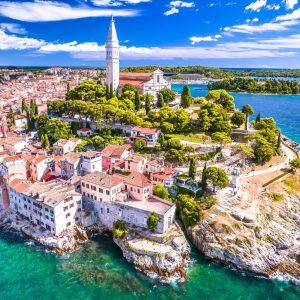
\includegraphics[width=0.25\textwidth]{rovinj.png} &
        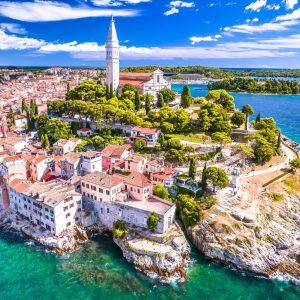
\includegraphics[width=0.125\textwidth]{rovinj.png} &
        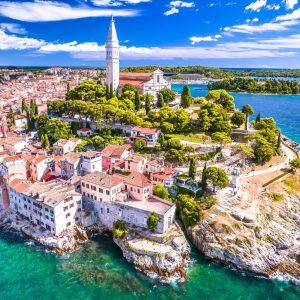
\includegraphics[width=0.1875\textwidth]{rovinj.png} &
        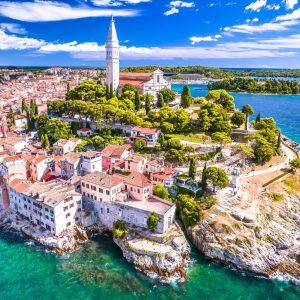
\includegraphics[width=0.25\textwidth, angle=45]{rovinj.png} \\
        \hline
        \textbf{Original Image} & \textbf{Rotated 90$^\circ$} & \textbf{Rotated 180$^\circ$} & \textbf{Scaled 125\%} \\
        \hline
        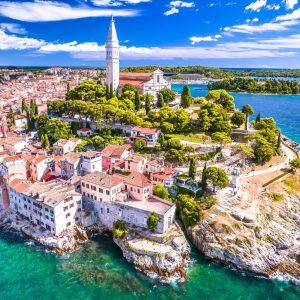
\includegraphics[width=0.25\textwidth]{rovinj.png} &
        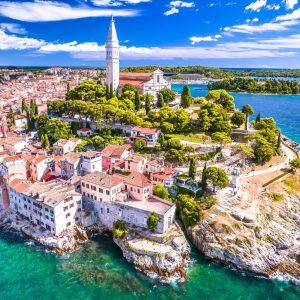
\includegraphics[width=0.25\textwidth, angle=90]{rovinj.png} &
        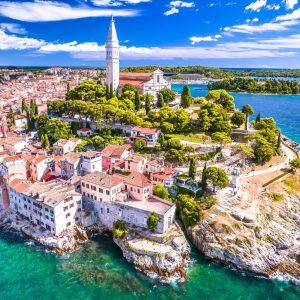
\includegraphics[width=0.25\textwidth, angle=180]{rovinj.png} &
        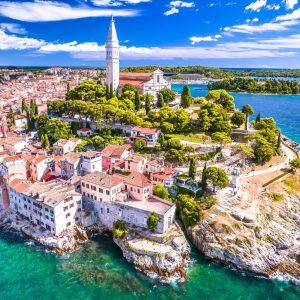
\includegraphics[width=0.3125\textwidth]{rovinj.png} \\
        \hline
    \end{tabular}
    \label{tab:image_table}
\end{table}

\end{document}
